\begin{center}
  \textsf{Листок 7.}
\end{center}
\vspace{0.01mm}
\nopagebreak[2]

\taskpic{ Два одинаковых кубика с длиной ребра $b$ массой $m$ каждый
  стоят на горизонтальном столе, на расстоянии $b$ друг от друга. Между
  ними помещён рычаг длиной $2^{3/2}b$ с пренебрежимо малой
  массой. Коэффициент трения между поверхностями кубиков и столом
  $k$. Коэффициент трения между рычагом и кубиками очень большой в точке
  $A$ и очень маленький в точке $C$. В точке $B$ приложена сила $F$,
  направленная перпендикулярно рычагу как показано на
  рисунке. Определите, какой из кубиков сдвигается раньше, если
  постепенно увеличивать силу $F$.  }{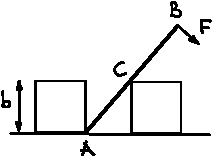
\includegraphics[width=4cm]{p09_26.pdf}}

\taskpic{ Однородный стрежень длиной $l$ опирается о пол и
  ступеньку. Коэффициент трения между стержнем и полом равен 1, трения
  между стержнем и ступенькой нет. При какой высоте ступеньки стержень
  может находиться в равновесии, если угол $\alpha = \pi /4$?
}{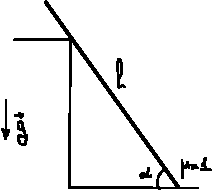
\includegraphics[width=4cm]{p09_27.pdf}}

\taskpic{ В системе, изображённой на рисунке, трение в блоках и между
  другими поверхностями отсутствует. Если грузу массой $m$ позволить
  двигаться, то за какое время он достигает подставки? Начальная
  скорость груза равна 0, начальное расстояние от груза до подставки
  $h$, нить невесомая и нерастяжимая. Масса подставки $M$.
}{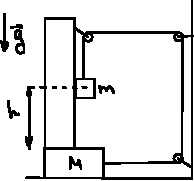
\includegraphics[width=4cm]{p09_28.pdf}}

\taskpic{ Найдите ускорение грузов, если масса каждого груза равна
  $m$. Массами нитей и блоков пренебречь, нити нерастяжимы, трение
  отсутствует.
}{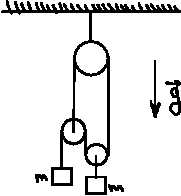
\includegraphics[width=4cm]{p09_29.pdf}}
